\documentclass{standalone}
\usepackage{tikz}

\begin{document}
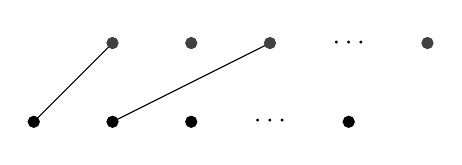
\begin{tikzpicture}
	%\draw[help lines] (0,-1) grid (\n+3,2);
	\def\n{4};
	\draw (1,0) -- (2,1);
	\draw (2,0) -- (4,1);
	\foreach \x in {1,...,\numexpr\n-1\relax}{
		\filldraw[black] (\x,0) circle (2pt);
		\filldraw[darkgray] (\x+1,1) circle (2pt);
	}
	\node at (\n,0) {$\cdots$};
	\node at (\n+1,1) {$\cdots$};
	\filldraw[black] (\n+1,0) circle (2pt);
	\filldraw[darkgray] (\n+2,1) circle (2pt);
\end{tikzpicture}
\end{document}
